%!TEX TS-program = xelatex
\documentclass[a4paper]{article}
\usepackage[a4paper, mag=1000, left=2.5cm, right=1cm, top=2cm, bottom=2cm, headsep=0.7cm, footskip=1cm]{geometry}
\usepackage[utf8]{inputenc}
\usepackage[english,russian]{babel}
\usepackage{multirow}
\usepackage{graphicx}
\usepackage{listings}
%\usepackage[colorlinks]{hyperref}

\usepackage{enumitem}

\usepackage{fontspec}
\setmainfont{Times New Roman}
\setsansfont{Arial}
\setmonofont{Courier New}
\newfontfamily\cyrillicfont[Script=Cyrillic]{Times New Roman}
\newfontfamily\cyrillicfontsf[Script=Cyrillic]{Arial}
\newfontfamily\cyrillicfonttt[Script=Cyrillic]{Courier New}
\usepackage{polyglossia}
\setdefaultlanguage{russian}
\usepackage{listings}

\lstdefinestyle{CppCodeStyle}{
	basicstyle=\footnotesize\ttfamily,
	language={[ANSI]C++},
	keywordstyle=\bfseries,
	showstringspaces=false,
	morekeywords={include, printf},
	commentstyle={},
	escapeinside=§§,
	escapebegin=\begin{russian}\commentfont,
		escapeend=\end{russian},
}
\newcommand{\commentfont}{\ttfamily}

\begin{document}
	\def\contentsname{Содержание}
	
	% Оформление титульного листа
	\begin{titlepage}
		\begin{center}
			\textbf{Московский Авиационный Институт\\[10mm]}
				Институт №3 \\
				Программная инженерия \\
				Кафедра 304 \\
			
			\vfill
			
			\textbf{Отчёт по лабораторной работе \\ 
				по учебной дисциплине "Информационные технологии" \\
				на тему \\
				"Вычисление суммы бесконечного ряда" \\ [50mm]
			}
		\end{center}
		
		\hfill
		\begin{minipage}{.5\textwidth}
			Выполнили: студенты группы М3О-111Б-22 \\ [2mm] 
			Яковченко Н.Р. \\
			Деккер Сергей, Сергей, Серёга, извини \\
		\end{minipage}%
		\vfill
		\begin{center}
			Москва, \the\year\ г.
		\end{center}
	\end{titlepage}
	
	% Содержание
	\tableofcontents
	\newpage
	
	\section{Задание}
	
	\begin{center}
	\rule{\textwidth}{1pt} \\[2mm]
		\begin{tabular}{ lllll }
			\multicolumn{1}{l}{Кафедра 304} & \multicolumn{4}{r}{Курс: ИНФОРМАЦИОННЫЕ ТЕХНОЛОГИИ} \\[2mm]
			\multicolumn{3}{l}{Задание: \textbf{Вычисление суммы бесконечного числового ряда}} & & \\[2mm]
		\end{tabular}
	\rule{\textwidth}{1pt} \\[2mm]
	Вариант №11
	\end{center}
	
	Определить с заданной точностью сумму членов бесконечного степенного ряда:
	
	$$ 1 + \displaystyle\sum_{n=1} \frac{x^{2n}}{(2n)!} = 1 + \frac{x^{2}}{2!} + \frac{x^{4}}{4!} + \frac{x^{6}}{6!} + ... $$
	
	Предусмотреть ввод точности и печать: количества просуммированных элементов, суммы, разности суммы и точного значения, которое равно:
	
	$$ \frac{e^{x} + e^{-x}}{2} = ch(x) $$
	
	\newpage
	
	\section{Схема алгоритма}
	
	\begin{center}
		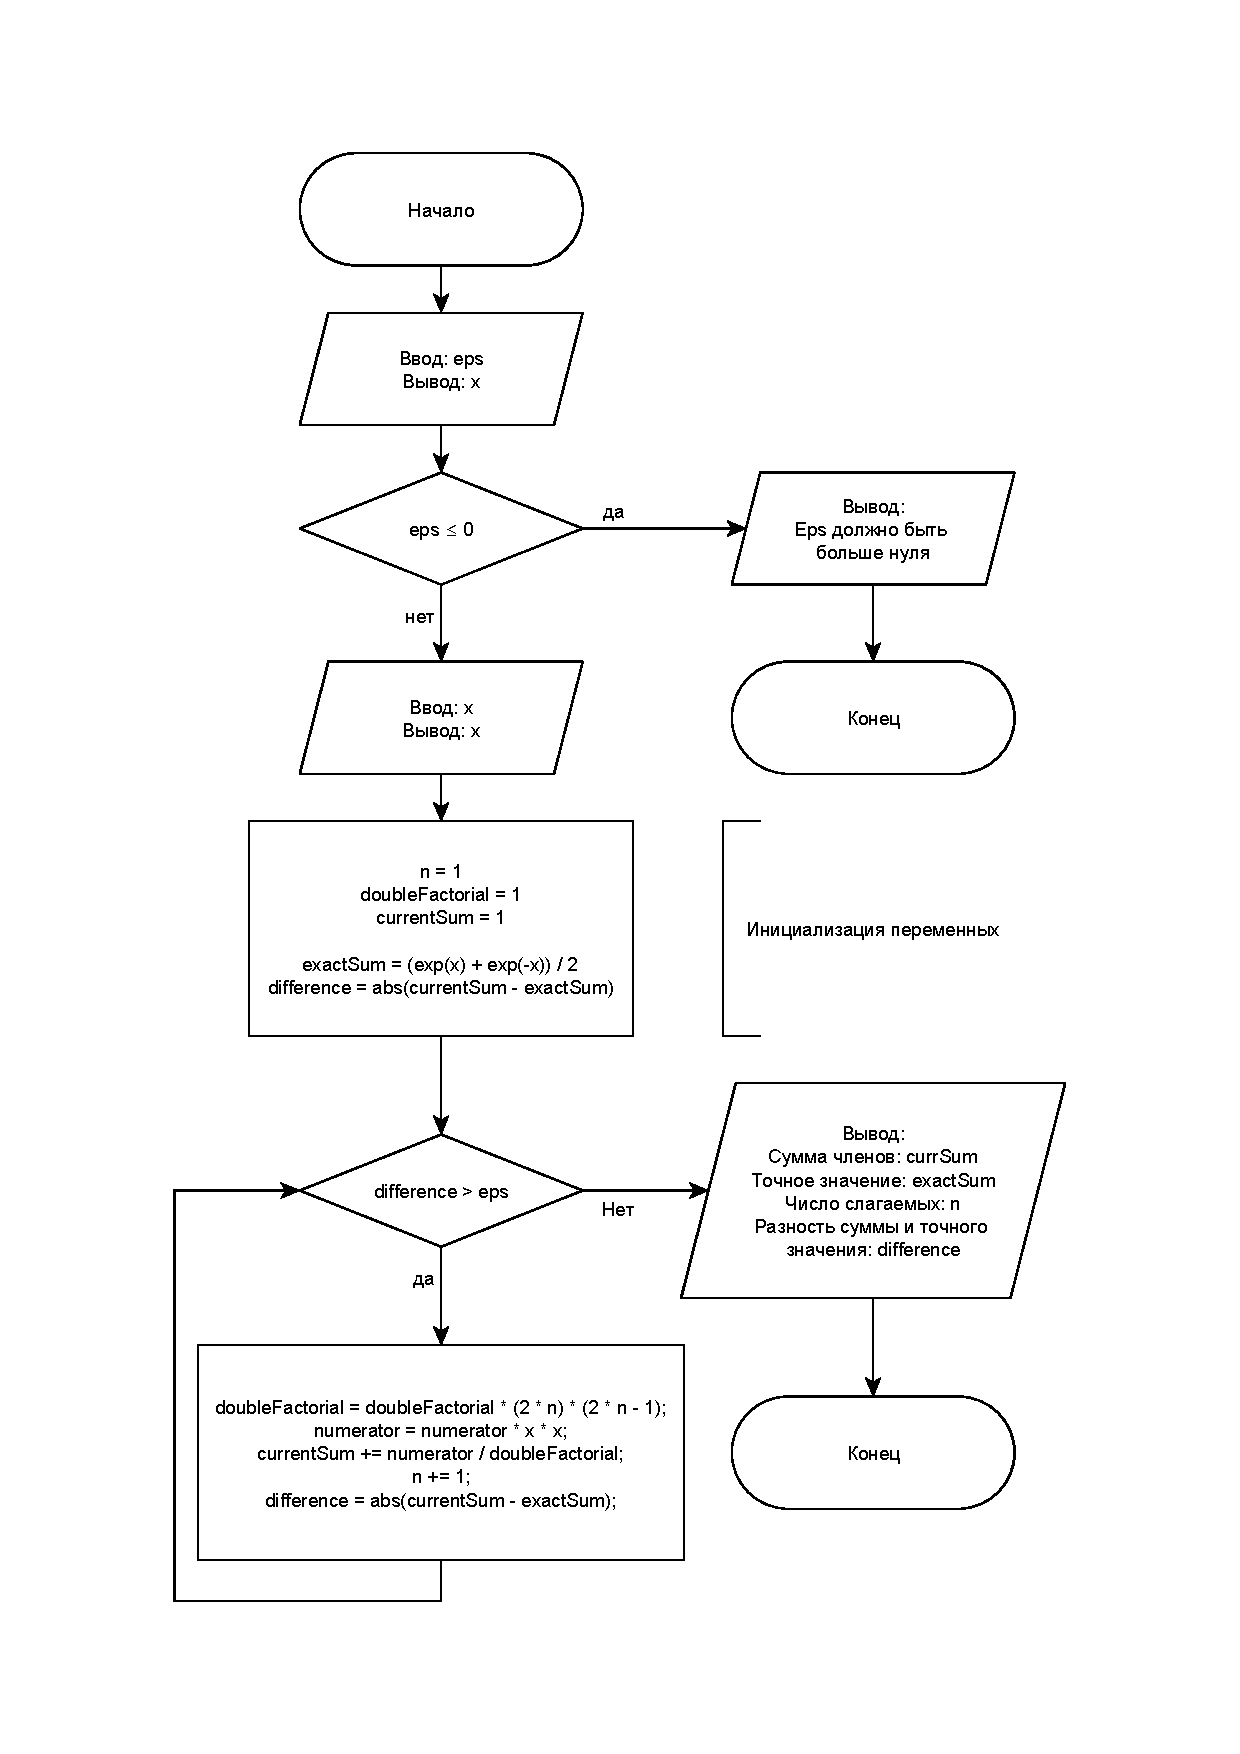
\includegraphics[width=\textwidth]{printed.pdf}
	\end{center}
	
	\newpage
	
	\section{Текст программы}
	
	\
	\begin{lstlisting}[style={CppCodeStyle}]
	// §Подключение библиотек§
	#include <iostream>
	#include <cmath>
	using namespace std;
	
	
	int main() // §Начало программы§
	{
		setlocale(LC_ALL, "rus"); // §Подключение русского языка§
		
		int n;                    // §Число слагаемых§
		unsigned long long doubleFactorial; // §Текущее значение удвоенного факториала§
		double difference;        // §Разность текущей и точной сумм§
		double currentSum;        // §Сумма§
		double exactSum;          // §Точное значение суммы§
		double x;                 // §Переменная§
		double eps;               // §Точность§
		double numerator;         // §Числитель§
		
		cout << "Введите точность: ";
		cin >> eps;               // §Ввод точности§
		cout << eps << endl;      // §Эхо-печать§
		
		if (eps <= 0)             // §Валидация входящих данных§
		{
			// §Вывод сообщения об ошибке§
			cout << "§Заданная точность должна быть больше нуля§" << endl; 
			// §Завершение работы программы в случае некорректности введённых данных§
			return 1;
		}
		
		cout << "Введите X: ";
		cin >> x;                 // §Ввод переменной x§
		cout << x << endl;        // §Эхо-печать§
		
		// §Инициализация переменных§
		n = 1;
		doubleFactorial = 1;
		currentSum = 1;
		numerator = 1;
		
		exactSum = (exp(x) + exp(-x)) / 2;       §// Подсчёт точной суммы§
		difference = abs(currentSum - exactSum); §// Подсчёт разности§
		
		while (difference > eps)  // §Начало цикла§
		{
			// §Вычисление суммы ряда§
			doubleFactorial = doubleFactorial * (2 * n) * (2 * n - 1);
			numerator = numerator * x * x;
			currentSum += numerator / doubleFactorial;
			n += 1;
			difference = abs(currentSum - exactSum);
		} // §Конец цикла§
		
		// §Вывод значений переменных§
		cout << "§Сумма членов: §" << currentSum << endl;
		cout << "§Точное значение: §" << exactSum << endl;
		cout << "§Число слагаемых: §" << n << endl;
		cout << "§Разность суммы и точного значения: §" << difference << endl;
		return 0; // §Возврат значения 0§
	}
	
	\end{lstlisting}
	\newpage
	
	\section{Тесты}
	\subsection{Некорректные тесты}
	
	\begin{enumerate}[label=\textbf{Тест \arabic*}]
		\item Цель: проверить работу программы на границе некорректной области \\
		Исходные данные: eps = 0 \\
		Ожидаемый результат: Заданная точность должна быть больше нуля \\
		Полученный результат:
		
		\begin{figure}[h]
			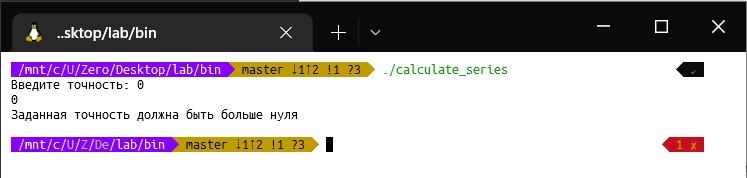
\includegraphics[width=\textwidth,trim=0.5mm 0 0 0.5mm,clip]{tests/test0.png}
		\end{figure}
	
		Вывод по тесту: Полученный результат совпал с ожидаемым. Тест ошибок не выявил.
		\vspace{5mm}
		
		\item Цель: проверить работу программы на границе некорректной области \\
		Исходные данные: eps = -1.02 \\
		Ожидаемый результат: Заданная точность должна быть больше нуля \\
		Полученный результат:
		
		\begin{figure}[h]
			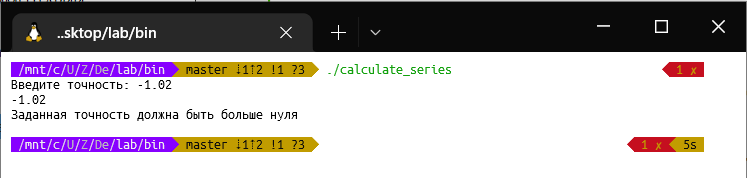
\includegraphics[width=\textwidth,trim=0.5mm 0 0 0.5mm,clip]{tests/test-1.02.png}
		\end{figure}
	
		Вывод по тесту: Полученный результат совпал с ожидаемым. Тест ошибок не выявил.
	\end{enumerate}
	
	\subsection{Корректные тесты}
	\begin{enumerate}[label=\textbf{Тест \arabic*}]
		\item Цель: проверить работу цикла по расчёту суммы ряда при высокой погрешности \\
		Исходные данные: eps = 100, x = 1 \\
		
		\begin{tabular}{l l}
			Ожидаемый результат: & Сумма членов: 1 \\
			& Точное значение: 1,5308 \\
			& Число слагаемых: 1 \\
			& Разность суммы и точного значения: 0,5308 \\[4mm]
		\end{tabular}
	
		Полученный результат:
		
		\begin{figure}[h]
			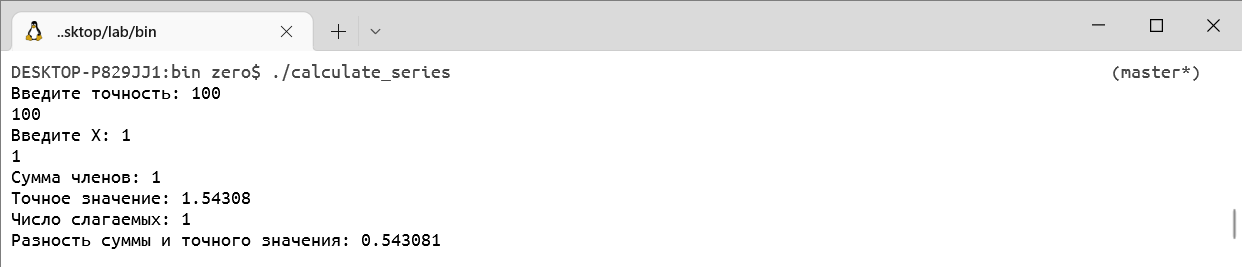
\includegraphics[width=\textwidth,trim=0.5mm 0 0 0.5mm,clip]{tests/test100.png}
		\end{figure}
		
		Вывод по тесту: Полученный результат совпал с ожидаемым. Тест ошибок не выявил.
		\newpage
		
		\item Цель: проверить работу цикла по расчёту суммы ряда \\
		Исходные данные: eps = 0.001, x = 3 \\
		
		\begin{tabular}{l l}
			Ожидаемый результат: & Сумма членов: 10,0676 \\
			& Точное значение: 10,0677 \\
			& Число слагаемых: 7 \\
			& Разность суммы и точного значения: $\approx 0,00006$ \\[4mm]
		\end{tabular}
		
		\begin{tabular}{l|l|l|l}
			n & currentSum & exactSum & difference  \\
			1 &  1  &\multirow{7}{*}{10,06766}& 9,06766 \\
			2 &  5,5  &       & 4,56766 \\
			3 &  8,875  &     & 1,19266 \\
			4 &  9,8875  &    & 0,18016 \\
			5 &  10,05022 &   & 0,01744 \\
			6 &  10,0665  &   & 0,00116 \\
			7 &  10,0676  &   & 0,00006 \\
		\end{tabular}
		
		\hspace{3mm}
		Полученный результат:
		
		\begin{figure}[h]
			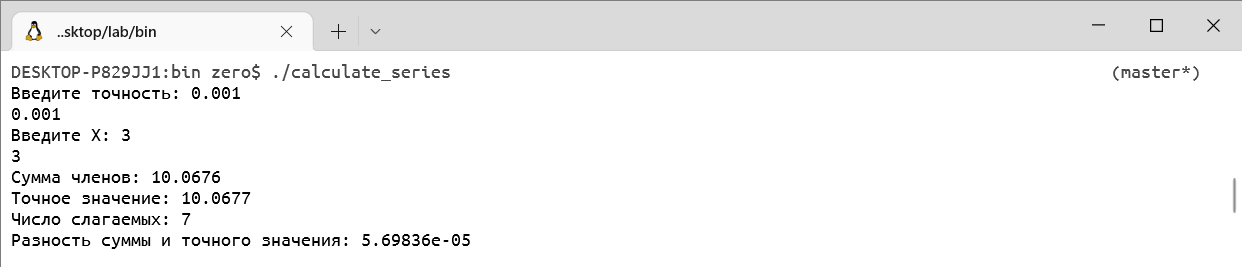
\includegraphics[width=\textwidth,trim=0.5mm 0 0 0.5mm,clip]{tests/test0.001.png}
		\end{figure}
		
		Вывод по тесту: Полученный результат совпал с ожидаемым. Тест ошибок не выявил.
		\newpage
		
		\item Цель: проверить работу цикла по расчёту суммы ряда \\
		Исходные данные: eps = 50, x = 10 \\
		
		\begin{tabular}{l l}
			Ожидаемый результат: & Сумма членов: 11002,4 \\
			& Точное значение: 11013.2 \\
			& Число слагаемых: 11 \\
			& Разность суммы и точного значения: $\approx 10,8$ \\[4mm]
		\end{tabular}
		
		\begin{tabular}{l|l|l|l}
			n & currentSum & exactSum & difference  \\
			1 &  1  &\multirow{11}{*}{11013.2}& 11012.2 \\
			2 &  51  &        & 10962,2 \\
			3 &  467,6  &     & 10545,6 \\
			4 &  1856,5  &    & 9156,7 \\
			5 &  4436,7 &     & 6576,5 \\
			6 &  7092,4  &    & 3920,8 \\
			7 &  9180,1  &    & 1833,1 \\
			8 & 10327,19 &    & 686,01 \\
			9 & 10805,1 &     & 208,1 \\
			10 & 10961,3 &    & 51,9 \\
			11 & 11002,4 &    & 10,8 \\
		\end{tabular}
		
		\hspace{3mm}
		Полученный результат:
		
		\begin{figure}[h]
			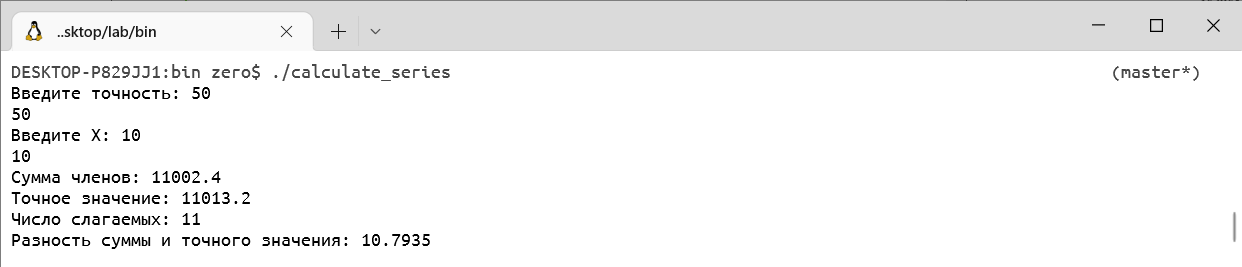
\includegraphics[width=\textwidth,trim=0.5mm 0 0 0.5mm,clip]{tests/test50.png}
		\end{figure}
		
		Вывод по тесту: Полученный результат совпал с ожидаемым. Тест ошибок не выявил.
	\end{enumerate}
	
\end{document}